\appendix

\section{Full Leaderboard}
\label{app:leaderboard}
Table~\ref{tab:leaderboard} reports \(\mathrm{pass}^3\) with 95\% confidence
intervals for all 24 models on the 750-task slice, the values summarized by
the heatmap in \S\ref{sec:results:main}.

\begin{table}[h]
  \centering
  \small
  \begin{tabular}{llr}
    \toprule
    Model & Group & \(\mathrm{pass}^3\) (\%, 95\% CI) \\
    \midrule
    qwen3.7-max & API & 51.2 \, [47.6, 54.8] \\
    glm-5.1 & API & 50.3 \, [46.7, 53.8] \\
    deepseek-v4-pro & API & 46.4 \, [42.9, 50.0] \\
    minimax-m3 & API & 42.4 \, [38.9, 46.0] \\
    claude-haiku-4.5 & API & 41.1 \, [37.6, 44.6] \\
    kimi-k2.6 & API & 40.7 \, [37.2, 44.2] \\
    grok-4.3 & API & 31.6 \, [28.4, 35.0] \\
    gpt-5.4-mini & API & 25.7 \, [22.7, 29.0] \\
    \midrule
    qwen3.6-35b & local & 48.5 \, [45.0, 52.1] \\
    gemma4-31b & local & 42.5 \, [39.0, 46.1] \\
    qwen3.5-4b & local & 27.3 \, [24.3, 30.6] \\
    granite-3b & local & 22.5 \, [19.7, 25.7] \\
    gemma4-e4b & local & 22.1 \, [19.3, 25.2] \\
    qwen3-8b & local & 22.1 \, [19.3, 25.2] \\
    nemotron-nano-4b & local & 21.9 \, [19.1, 25.0] \\
    qwen2.5-7b & local & 21.1 \, [18.3, 24.1] \\
    gemma4-e2b & local & 20.1 \, [17.4, 23.2] \\
    xlam2-8b & local & 19.5 \, [16.8, 22.4] \\
    toolace2-8b & local & 17.5 \, [14.9, 20.3] \\
    qwen2.5-3b & local & 16.9 \, [14.4, 19.8] \\
    hermes3-8b & local & 13.2 \, [11.0, 15.8] \\
    ministral3-3b & local & 12.4 \, [10.2, 14.9] \\
    hammer2.1-7b & local & 9.7 \, [7.8, 12.1] \\
    smollm3-3b & local & 7.2 \, [5.6, 9.3] \\
    \bottomrule
  \end{tabular}
  \caption{Full leaderboard: \(\mathrm{pass}^3\) and 95\% confidence
    intervals over the 750-task slice, for the 8 API-served and 16
    locally-served models.}
  \label{tab:leaderboard}
\end{table}

\section{Task Categories}
\label{app:categories}
The 15 categories are assembled in three tiers. A category controls only the
\emph{seed} tool-set; the explorer still solves the goal forward.

\noindent\textbf{Base relationships (6).} An anchor tool is chosen and a
related seed set is sampled by tool-relationship; these samplers double as the
evaluation-time distractor selectors.
\begin{itemize}
  \item \emph{random}: a uniform-random seed set; the neutral baseline.
  \item \emph{hard-negative}: tools whose descriptions are most similar to the
    anchor (near-duplicates removed), probing look-alike confusion.
  \item \emph{cross-domain}: similar tools whose server domain (tags) differs
    from the anchor's, probing wrong-domain look-alikes.
  \item \emph{same-name}: tools with the same name on a \emph{different} server
    (plus near-collisions), the server-attribution primitive.
  \item \emph{sibling}: other tools on the \emph{same} server, probing
    intra-server confusion.
  \item \emph{stratified}: a round-robin mix of the five above.
\end{itemize}
\noindent\textbf{Corner cases (7).} A base relationship plus a goal framing
that demands a specific challenge.
\begin{itemize}
  \item \emph{long-similar-chain}: a multi-step task chaining several similar
    tools in sequence.
  \item \emph{homonym-trap}: a capability exposed under the same tool name on
    several servers, requiring the intended source.
  \item \emph{decoy}: one tool is correct while a similar tool is a tempting
    wrong shortcut.
  \item \emph{prerequisite-strict}: a strict required order, where an earlier
    output is a prerequisite for a later step.
  \item \emph{recovery-required}: the obvious first tool is insufficient and a
    second tool is needed to recover.
  \item \emph{destructive-adjacent}: a read-only task on a server that also
    exposes destructive tools that must not be used.
  \item \emph{ambiguous-intent}: a deliberately vague request several tools
    could each plausibly satisfy.
\end{itemize}
\noindent\textbf{Cross-server specials (2).} Seeded from curated sources
rather than the anchor sampler.
\begin{itemize}
  \item \emph{cross-server-alternative}: seeded from same-name tool groups
    spanning $\geq 2$ servers; the task must name the intended server.
  \item \emph{complementary}: seeded from output$\rightarrow$input
    data-dependency edges; one tool's output feeds the next tool's input.
\end{itemize}

\section{Framework Configuration}
\label{app:config}
We report the configuration that produced the released results; the framework
exposes every value as a parameter.

\noindent\textbf{Generation.} Tasks are generated forward over all 15
categories. For each, an anchor tool is selected and the category's
relationship sampler picks the seed set, whose size is set by a complexity
level (simple~$=2$, medium~$=4$, hard~$=6$ tools) swept to span short and long
chains; phrasing is persona-seeded for linguistic diversity. Authorship is
spread across many model families, with the explorer and the distiller
constrained to \emph{different} families to limit self-preference. The
explorer runs with a 12-turn budget; the distiller emits the task
specification deterministically (temperature~0) under a large token budget so
that reasoning models do not truncate the structured output. Each choice
isolates a difficulty axis or removes a confound: the complexity sweep gives a
controlled difficulty axis, multi-family authorship avoids a single-generator
monoculture, the explorer/distiller family split limits self-preference, and
personas add phrasing diversity.

\noindent\textbf{Evaluation.} Candidates are scored under deterministic replay
against each task's recorded world, so every model faces an identical
environment. Each task is run three times and counts as solved only if all
three runs pass (\(\mathrm{pass}^3\)). The candidate is offered a
\emph{target} tool pool: the tools the task needs plus eight distractors, half
of them same-name tools on other servers (the rest near-misses), which gives a
controlled, identical-across-models server-attribution stress. Tool
descriptions are presented as written and all tools are exposed directly
(flat), so the headline measures the agent rather than a description
normalizer or a retriever. The headline uses Tier-1 deterministic effect
scoring; a Tier-2 effect-equivalence judge (fuzzy threshold~0.75) is an
available option that upgrades only failed tool-effect checkpoints and never
reads the final answer. Description-normalization, tool-exposure architecture,
and the alternative-tool density are framework parameters reserved for
controlled ablations.

\section{Prompts}
\label{app:prompts}
We reproduce the system prompts verbatim.

\noindent\textbf{Goal generation.}
{\footnotesize
\begin{verbatim}
You are designing realistic user goals for an MCP-agent benchmark.

You will be shown one or more MCP servers, each with:
  - server_id (use this exact string in `servers`)
  - dynamism class (static / live_read / stateful_write)
  - sandbox_resources: a list of concrete resources we HAVE actually set up
    for this server (paths, file specs, env-provided IDs). Empty means we
    have set up nothing - design the goal around discovery/exploration of
    whatever the tools expose by default.
  - tool surface: name + short description + input schema

Your job: call `emit_goals` exactly once with N realistic user goals that
exercise these servers. Hard rules:

  1. Each goal is a natural-language request a real user might make. Do NOT
     write "call tool X with args Y" - write the request the user would
     actually voice.
  2. Each goal must be solvable using ONLY the servers shown.
  3. NEVER INVENT concrete external resources (file paths, IDs, keys, URLs).
     If sandbox_resources is empty, design the goal around DISCOVERY instead.
  4. When sandbox_resources is non-empty, use those exact strings verbatim.
  5. Vary complexity: mix single-call and multi-step goals (2-5 calls).
  6. For stateful_write servers WITH sandbox_resources, prefer verifiable
     effects; WITHOUT them, prefer read-only / discovery goals.
  7. For cross-server goals, design genuine data dependencies.
  8. Avoid destructive operations unless the task is an undo/recovery scenario.
  9. Choose tags from a fixed list (shallow, single-server, cross-server,
     deep, runtime-branching, recovery, read-only-usage, parallel-calls,
     discovery).
\end{verbatim}
}
A per-call persona block and the category framing are appended at request
time.

\noindent\textbf{Exploration / candidate agent.}
{\footnotesize
\begin{verbatim}
You are an exploration agent driving MCP tools to satisfy a user goal.

Rules:
- Call tools to make progress. Do not invent results - use the tools.
- Each tool name is namespaced as <server_id>__<tool_name>. Use exactly that.
- When the goal is satisfied, respond with a short summary and stop.
- If a tool errors, read the error, adjust arguments, and try again.
- Prefer the simplest sequence of calls that achieves the goal.
\end{verbatim}
}

\noindent\textbf{Distillation.}
{\footnotesize
\begin{verbatim}
You are compiling an MCP tool-use trace into a benchmark task specification.

You will be shown the goal, the successful tool calls (in order, with args
and result previews), and the available tools per server.

Call `emit_task_spec` exactly once, with:
  - prompt: a fuzzy user request; strip explicit tool names but PRESERVE
    concrete context (paths, file names, URLs, identifiers).
  - checkpoints: at least one, each either
      tool_effect    - a tool from an equivalence set must have been called
                       successfully, optionally matching arg predicates
                       (must_include = exact equality; must_match = richer
                       per-key matchers for variable/derived values).
      value_produced - a tool result (or final message) must contain
                       certain substrings.
  - minefields: things the agent must NOT do (often empty for read-only).
  - notes: anything ambiguous or any alternative valid path.

Be tight: do not invent checkpoints the trace does not justify. When two
tools equally satisfy a checkpoint, list both in equivalence_set.
\end{verbatim}
}

\noindent\textbf{Tier-2 effect-equivalence judge.}
{\footnotesize
\begin{verbatim}
You are an effect-equivalence judge for an agent benchmark.

You will be shown one *failed* tool_effect checkpoint and the candidate's
successful tool calls. Decide ONE binary question: did the candidate achieve
the same *effect* the checkpoint requires, via any path?

Decision rules:
  - Default is NO; say YES only with clear evidence in the trace.
  - "Equivalent effect": an external observer could not tell the reference
    path from the alternative - same fact retrieved / record created / state
    mutated.
  - The final natural-language summary is NOT evidence on its own; a
    corresponding tool call is required.
  - When arg_predicate names a specific value, be strict.

Call `emit_equivalence_judgment` exactly once with your decision.
\end{verbatim}
}

\section{Accuracy versus Model Size}
\label{app:size}
Figure~\ref{fig:size} plots \(\mathrm{pass}^3\) against parameter count for
the locally-served models. The two largest lead, but below $\sim$30B
parameters size predicts accuracy only weakly: a 4B model outperforms every
7--8B model and, at a fixed 8B size, \(\mathrm{pass}^3\) ranges from 13\% to
22\%.

\begin{figure}[h]
  \centering
  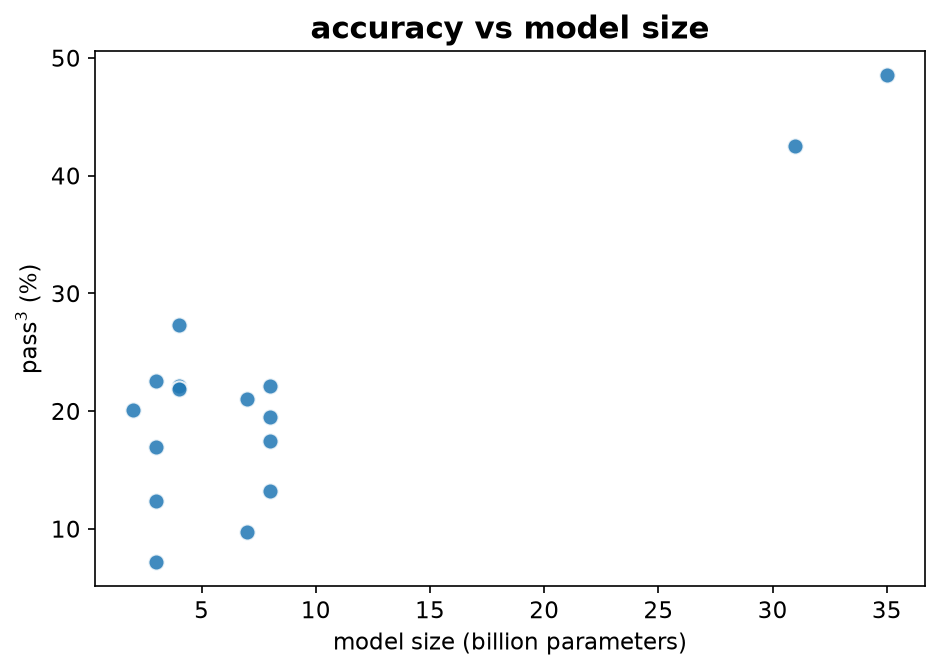
\includegraphics[width=\columnwidth]{figures/fig_size.png}
  \caption{Accuracy versus model size (locally-served models).}
  \label{fig:size}
\end{figure}
